\documentclass[aspectratio=169,10pt]{beamer}
% build: latexmk -xelatex -interaction=nonstopmode main.tex
% figures: see make_figs.py (session T only)

\usetheme{metropolis}
\metroset{block=fill, numbering=fraction, progressbar=frametitle, sectionpage=none}
\usepackage{appendixnumberbeamer}

\usepackage{fontspec}
% Fira from TeX Live, loaded by file name so it works without a system install
\setsansfont{FiraSans}[Extension=.otf, UprightFont=*-Book, BoldFont=*-SemiBold,
  ItalicFont=*-BookItalic, BoldItalicFont=*-SemiBoldItalic]
\setmonofont{FiraMono}[Extension=.otf, UprightFont=*-Regular, BoldFont=*-Bold]

\usepackage{amsmath,amssymb}
\usepackage{booktabs}
\usepackage{graphicx}
\usepackage{tikz}
\usetikzlibrary{arrows.meta, positioning, decorations.pathreplacing, calc}

% palette (same as the seminar decks)
\definecolor{fit}{HTML}{1B7F79}     % learned from the training fold
\definecolor{mix}{HTML}{9A6A00}     % same as MixNet
\definecolor{qcol}{HTML}{7A3E9D}
\newcommand{\fitc}[1]{\textcolor{fit}{#1}}
\newcommand{\mixc}[1]{\textcolor{mix}{#1}}
\newcommand{\lec}[1]{\unskip\nobreak\hspace{0.35em}\mbox{\scriptsize\textcolor{gray}{[lecture p.#1]}}}
\newcommand{\uu}[1]{\texttt{#1}}

\newenvironment{keybox}[1][Key point]{%
  \setbeamercolor{block title}{bg=fit,fg=white}%
  \setbeamercolor{block body}{bg=fit!8,fg=black}%
  \begin{block}{\small #1}\small}{\end{block}}
\newenvironment{qbox}[1][Note]{%
  \setbeamercolor{block title}{bg=qcol,fg=white}%
  \setbeamercolor{block body}{bg=qcol!8,fg=black}%
  \begin{block}{\small #1}\small}{\end{block}}

\setbeamerfont{footnote}{size=\tiny}

\title{Part 1: Preprocessing}
\subtitle{Filter-bank CSP + band power in short time windows}
\author{} % TODO: team names
\institute{\footnotesize ML Frontiers, VISTEC \textperiodcentered\ BCIC IV-2a, left vs right hand MI}
\date{}

\begin{document}
\maketitle
% !TEX root = main.tex
\section{Preprocessing}

% ---------------------------------------------------------------------------
\begin{frame}{Why not just use CSP, or MixNet's input?}
\begin{columns}[T]
\begin{column}{0.40\textwidth}
\begin{itemize}\small
\item MI shows up as \alert{ERD/ERS in Mu and beta}, around C3/C4 \lec{51}
\item Classic CSP keeps one log-variance per trial, so it \alert{throws away the timing} inside the trial \lec{62}
\item MixNet keeps the whole CSP time series \lec{63}: 7{,}200 numbers per trial, learned from only $\sim$115 training trials
\end{itemize}
\end{column}
\begin{column}{0.58\textwidth}
\footnotesize\setlength{\tabcolsep}{4pt}
\begin{tabular}{@{}lccc@{}}
\toprule
 & \mixc{Classic FBCSP} & \mixc{MixNet} & \fitc{Ours} \\
\midrule
Keeps timing      & no   & all 400 samples & 15 windows \\
Shape per trial   & 36   & $18\times400$  & $36\times15$ \\
Numbers per trial & 36   & 7{,}200        & 540 \\
\bottomrule
\end{tabular}

\medskip
\begin{keybox}[Hypothesis]
Band power in \alert{short time windows} keeps the timing of ERD/ERS, at a size a small model can learn from $\sim$115 trials.
\end{keybox}
\end{column}
\end{columns}
\end{frame}

% ---------------------------------------------------------------------------
\begin{frame}{Pipeline: four steps, two of them learned}
\centering
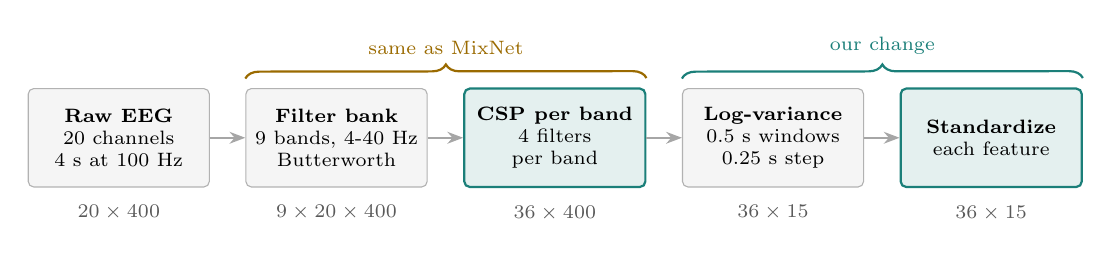
\begin{tikzpicture}[
  box/.style={draw=gray!60, fill=gray!8, rounded corners=2pt, align=center,
              minimum width=2.3cm, minimum height=1.25cm, font=\scriptsize},
  learn/.style={box, draw=fit, fill=fit!12, thick},
  arr/.style={-{Stealth[length=2mm]}, thick, gray!70},
  shp/.style={font=\scriptsize, text=gray!70!black}]
\node[box]                        (raw) {\textbf{Raw EEG}\\20 channels\\4 s at 100 Hz};
\node[box,   right=0.45cm of raw] (fb)  {\textbf{Filter bank}\\9 bands, 4-40 Hz\\Butterworth};
\node[learn, right=0.45cm of fb]  (csp) {\textbf{CSP per band}\\4 filters\\per band};
\node[box,   right=0.45cm of csp] (lv)  {\textbf{Log-variance}\\0.5 s windows\\0.25 s step};
\node[learn, right=0.45cm of lv]  (std) {\textbf{Standardize}\\each feature};
\foreach \a/\b in {raw/fb, fb/csp, csp/lv, lv/std} \draw[arr] (\a) -- (\b);
\node[shp, below=1mm of raw] {$20\times400$};
\node[shp, below=1mm of fb]  {$9\times20\times400$};
\node[shp, below=1mm of csp] {$36\times400$};
\node[shp, below=1mm of lv]  {$36\times15$};
\node[shp, below=1mm of std] {$36\times15$};
\draw[decorate, decoration={brace, amplitude=5pt}, thick, mix]
  ($(fb.north west)+(0,0.12)$) -- ($(csp.north east)+(0,0.12)$)
  node[midway, above=5pt, font=\scriptsize] {same as MixNet};
\draw[decorate, decoration={brace, amplitude=5pt}, thick, fit]
  ($(lv.north west)+(0,0.12)$) -- ($(std.north east)+(0,0.12)$)
  node[midway, above=5pt, font=\scriptsize] {our change};
\end{tikzpicture}

\medskip
\begin{columns}[T]
\begin{column}{0.55\textwidth}
\begin{keybox}[Teal boxes: fit on the training fold only]
\begin{itemize}
\item ``Fit CSP: training data only'' \lec{60}
\item ``Training-set per-channel standardization'' \lec{31}
\item Validation and session E only reuse the saved filters and mean/SD. A self-check in the code tests this.
\end{itemize}
\end{keybox}
\end{column}
\begin{column}{0.4\textwidth}
\begin{qbox}[Output per trial]
36 features (9 bands $\times$ 4 CSP filters) $\times$ 15 time windows, standardized
\end{qbox}
\end{column}
\end{columns}
\end{frame}

% ---------------------------------------------------------------------------
\begin{frame}{Our change: one log-variance per short window}
\begin{columns}[c]
\begin{column}{0.55\textwidth}
\centering
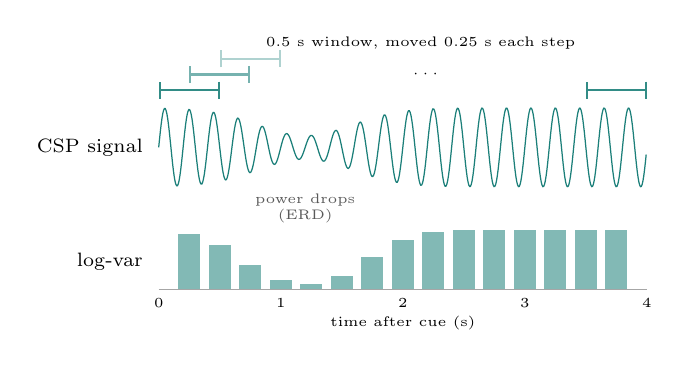
\begin{tikzpicture}[x=1.55cm, y=0.5cm]
  % one CSP component: power drops (ERD) about 1 s after the cue
  \draw[fit, line width=0.45pt] plot[domain=0:4, samples=600]
    (\x, {(1-0.7*exp(-((\x-1.2)/0.55)^2))*sin(360*5*\x)});
  \node[font=\tiny, text=gray!70!black, align=center] at (1.2,-1.55) {power drops\\(ERD)};
  \node[font=\scriptsize, anchor=east] at (-0.05,0) {CSP signal};
  % sliding windows
  \foreach \k/\c in {0/90, 1/60, 2/35} {
    \draw[fit!\c, thick, |-|] (0.25*\k, 1.45+0.4*\k) -- ++(0.5,0);
  }
  \draw[fit!90, thick, |-|] (3.5, 1.45) -- ++(0.5,0);
  \node[font=\tiny] at (2.2, 1.85) {$\cdots$};
  \node[font=\tiny, anchor=west] at (0.8, 2.65) {0.5 s window, moved 0.25 s each step};
  % one bar per window
  \foreach \k in {0,...,14} {
    \pgfmathsetmacro{\c}{0.25+0.25*\k}
    \pgfmathsetmacro{\h}{1.5*(1-0.7*exp(-((\c-1.2)/0.55)^2))^2}
    \fill[fit!55] (\c-0.09, -3.6) rectangle (\c+0.09, -3.6+\h);
  }
  \node[font=\scriptsize, anchor=east] at (-0.05,-2.9) {log-var};
  \draw[gray!70] (0,-3.6) -- (4,-3.6);
  \foreach \t in {0,...,4} \node[font=\tiny, below] at (\t,-3.6) {\t};
  \node[font=\tiny] at (2,-4.45) {time after cue (s)};
\end{tikzpicture}
\end{column}
\begin{column}{0.43\textwidth}
\begin{keybox}[Normalized log-variance]
For band $b$, CSP filter $i$, window $w$:
\[
f_{b,i,w} = \log \frac{\operatorname{var}(z_{b,i}[w])}{\sum_{j=1}^{4}\operatorname{var}(z_{b,j}[w])}
\]
\lec{59}
\end{keybox}
\begin{itemize}\small
\item $(400-50)/25+1 = 15$ windows in 4~s
\item This step learns nothing, so it cannot leak
\item Then each feature is standardized with the training-fold mean and SD \lec{31}
\end{itemize}
\end{column}
\end{columns}
\end{frame}

% ---------------------------------------------------------------------------
\begin{frame}{Quick LDA test: class information is not spread evenly in time}
\begin{columns}[c]
\begin{column}{0.58\textwidth}
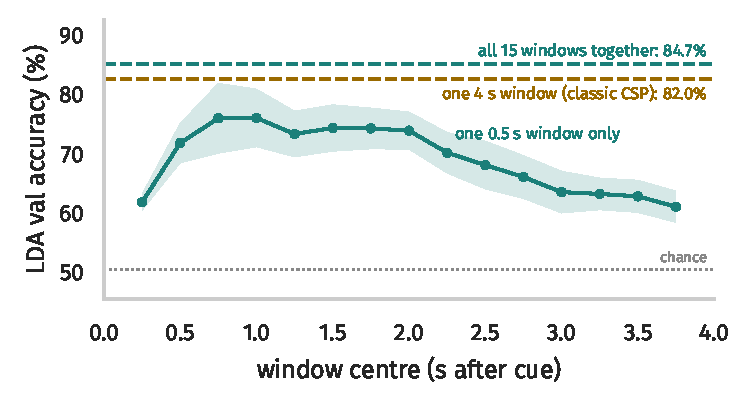
\includegraphics[width=\linewidth]{fig/acc_by_window.pdf}
\end{column}
\begin{column}{0.40\textwidth}
\begin{itemize}\footnotesize
\item \alert{One 0.5 s window} (36 numbers, one LDA per window): peaks at \mbox{0.75-1 s} (75.5\%), near 61\% at both ends
\item \mixc{One 4 s window} = whole trial, classic CSP (36 numbers): \mixc{82.0\%}
\item \fitc{All 15 windows together} = our features (540 numbers): \fitc{84.7\%}, better in 8 of 9 subjects
\end{itemize}
\end{column}
\end{columns}
\begin{qbox}[How we got these numbers]
\scriptsize
A simple shrinkage LDA, the classic classifier after CSP \lec{60}, trained on our features before building HWNet.
Same 5 folds as the real pipeline: fit on the training fold, score on the validation fold of session T, mean of 9 subjects (band = $\pm$1 SE).
Session E not used: \alert{not test results}, not comparable with MixNet.
\end{qbox}
\end{frame}

% ---------------------------------------------------------------------------
\begin{frame}{What the model sees: 36 features $\times$ 15 windows}
\begin{columns}[c]
\begin{column}{0.55\textwidth}
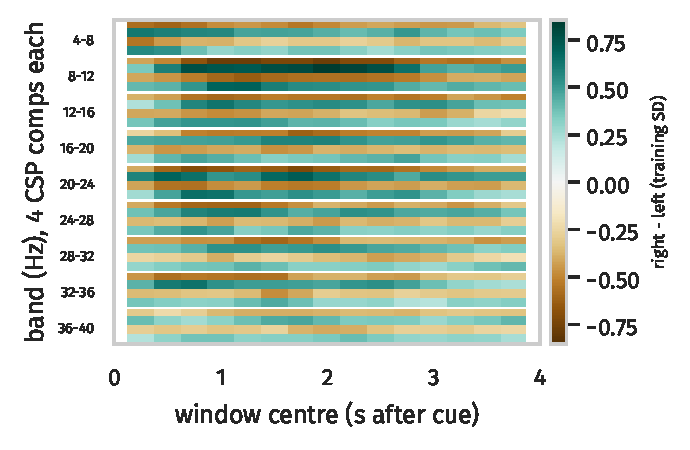
\includegraphics[width=\linewidth]{fig/feature_map.pdf}
\end{column}
\begin{column}{0.43\textwidth}
\begin{itemize}\small
\item Each cell: right minus left class mean, in training SD units
\item Strongest in \alert{\mbox{8-12 Hz} (Mu)} and \alert{\mbox{20-24 Hz} (beta)}, from about 0.5 to 2.5 s, the bands where ERD/ERS shows up \lec{51}
\item Rows alternate in sign because CSP takes filters from \alert{both ends}: one end has more power for left hand, the other for right \lec{57}
\end{itemize}
\begin{keybox}[Takeaway]
Each trial becomes \emph{which band}, \emph{which spatial filter} and \emph{when}, in 540 numbers.
\end{keybox}
\end{column}
\end{columns}
\vfill
{\tiny All 144 session T trials per subject, averaged over 9 subjects. Session E not used.\par}
\end{frame}

% ---------------------------------------------------------------------------
\appendix
\begin{frame}{Backup: settings and data notes}
\begin{columns}[T]
\begin{column}{0.56\textwidth}
\small
All settings live in \uu{experiments/prep\_HW.py}

\medskip
{\footnotesize\setlength{\tabcolsep}{4pt}
\begin{tabular}{@{}lll@{}}
\toprule
Setting & Ours & Ablation \\
\midrule
\uu{win\_len}, \uu{win\_step} & 0.5 s, 0.25 s & 4.0 s, 4.0 s (classic) \\
\uu{n\_components}            & 4             & 2 (MixNet size) \\
\uu{norm\_logvar}             & True          & False \\
\uu{bands}                    & 9 bands, 4-40 Hz & \\
\uu{order}                    & 5             & \\
\bottomrule
\end{tabular}}

\medskip
{\scriptsize Quick LDA check (validation, session T): ours 84.7\%, classic 82.0\%, \uu{norm\_logvar=False} 85.0\%, \uu{n\_components=2} not run yet.\par}
\end{column}
\begin{column}{0.42\textwidth}
\begin{qbox}[Data notes]
\begin{itemize}
\item 50 Hz line noise: removed. After resampling to 100 Hz it sits at the top edge, where every band filter blocks it
\item Drift and eye movement below 4 Hz: removed by the lowest band edge
\item Not removed: blinks in 4-8 Hz, muscle noise in beta, and trials marked as artifacts (2 to 36 of 144 per subject)
\end{itemize}
\end{qbox}
\end{column}
\end{columns}
\end{frame}

% ---------------------------------------------------------------------------
%  Walkthrough of one subject (figures: make_example_figs.py 3)
% ---------------------------------------------------------------------------
\newcommand{\exnote}{\vfill{\tiny Subject 3, session T only (144 trials, 72 per class). Example trials = the trial closest to its class mean. CSP and scaler fit on all session T trials of S3 for this picture; no accuracy is computed here.\par}}

\begin{frame}{S3 walkthrough (1/5): raw EEG, $20\times400$}
\begin{columns}[c]
\begin{column}{0.66\textwidth}
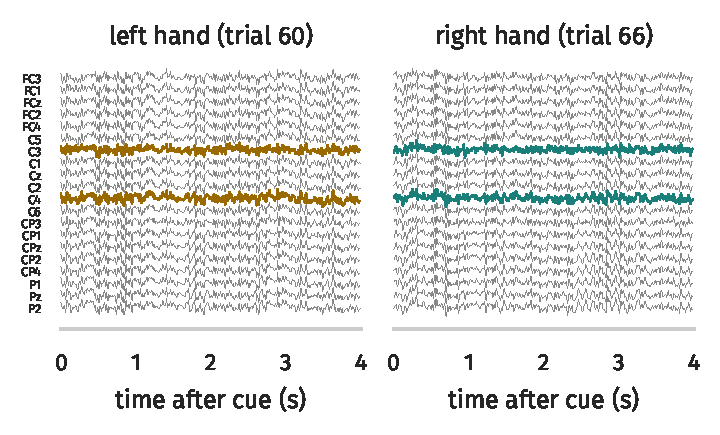
\includegraphics[width=\linewidth]{fig/ex_raw.pdf}
\end{column}
\begin{column}{0.32\textwidth}
\begin{itemize}\small
\item One \mixc{left hand} and one \fitc{right hand} trial: 20 channels, 4 s at 100 Hz
\item C3 and C4 (over the hand areas) in colour
\item By eye the two classes look the same: the difference is hidden in \alert{band power}
\end{itemize}
\end{column}
\end{columns}
\exnote
\end{frame}

\begin{frame}{S3 walkthrough (2/5): filter bank, $9\times20\times400$}
\begin{columns}[c]
\begin{column}{0.66\textwidth}
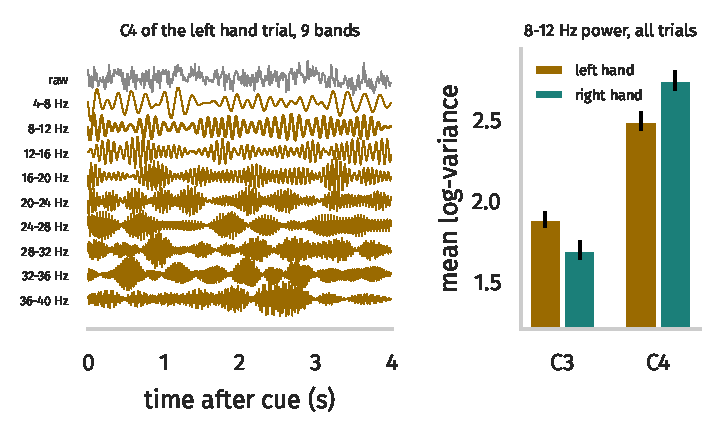
\includegraphics[width=\linewidth]{fig/ex_filterbank.pdf}
\end{column}
\begin{column}{0.32\textwidth}
\begin{itemize}\small
\item Left: C4 of the left hand trial split into 9 bands (each trace scaled on its own)
\item Right: 8-12 Hz power is lower at \alert{C4 for left hand} and lower at \alert{C3 for right hand}
\item That is contralateral ERD \lec{51}
\end{itemize}
\end{column}
\end{columns}
\exnote
\end{frame}

\begin{frame}{S3 walkthrough (3/5): CSP per band, $36\times400$ (8-12 Hz shown)}
\begin{columns}[c]
\begin{column}{0.66\textwidth}
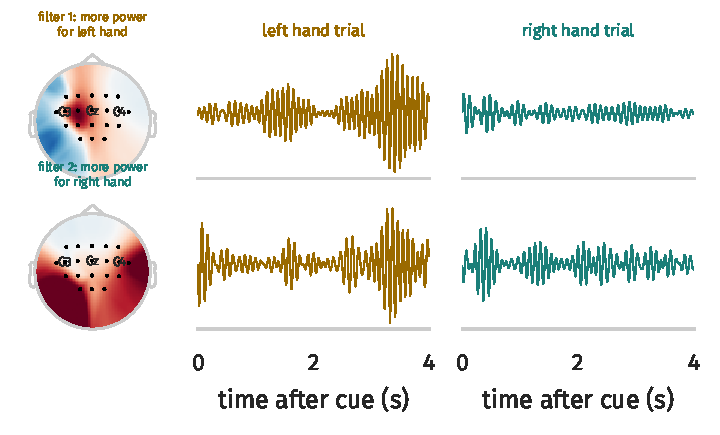
\includegraphics[width=\linewidth]{fig/ex_csp.pdf}
\end{column}
\begin{column}{0.32\textwidth}
\begin{itemize}\small
\item Maps: spatial pattern of each filter, i.e.\ where it looks \lec{58}
\item Filter 1 gives more power for left hand, filter 2 for right hand
\item Filter 1 shows the gap clearly in these two trials; filter 2 less so, single trials are noisy
\item 20 channels become 4 signals per band; time is untouched
\end{itemize}
\end{column}
\end{columns}
\exnote
\end{frame}

\begin{frame}{S3 walkthrough (4/5): windowed log-variance, $36\times15$}
\begin{columns}[c]
\begin{column}{0.62\textwidth}
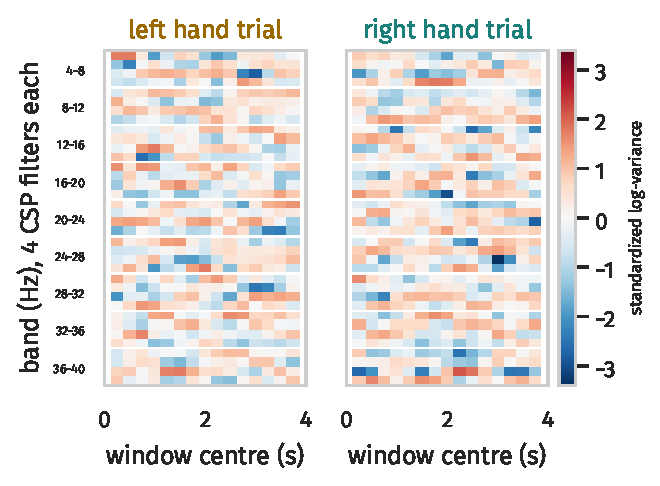
\includegraphics[width=\linewidth]{fig/ex_features.pdf}
\end{column}
\begin{column}{0.36\textwidth}
\begin{itemize}\small
\item The same two trials as the model sees them: 36 rows (9 bands $\times$ 4 filters) $\times$ 15 windows, standardized
\item One trial alone is noisy; the class difference shows up only across many trials (next slide)
\end{itemize}
\end{column}
\end{columns}
\exnote
\end{frame}

\begin{frame}{S3 walkthrough (5/5): do the features separate the classes?}
\centerline{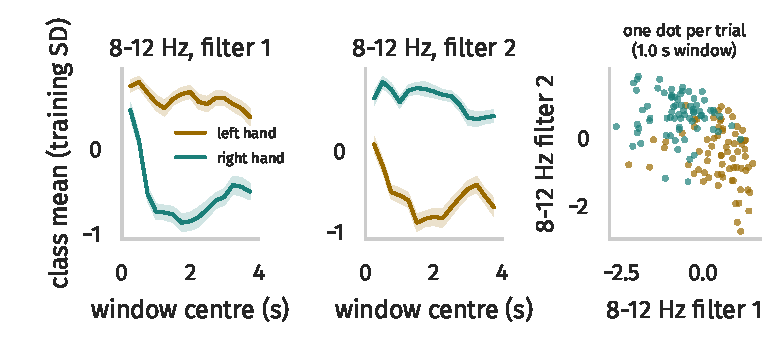
\includegraphics[width=0.78\linewidth]{fig/ex_separation.pdf}}
\begin{itemize}\footnotesize
\item Class means of the two 8-12 Hz filters: the gap is small right after the cue and grows within about 1 s, the timing our windows keep
\item Right: every trial at the 1.0 s window, using only 2 of the 540 numbers, already mostly separable
\item S3 is one of the easier subjects (quick LDA check: 95.8\%), so other subjects look less clean
\end{itemize}
\exnote
\end{frame}

\end{document}
